\chapter{Procedural assignments} \label{ch:behavioralModeling}
\chapterquote{That knowledge which purifies the mind and heart alone is true Knowledge, all else is only a negation of Knowledge.}{Ramakrishna Paramahansa}

\graphicspath{{Chapters/ProceduralAssignments/Figures/}}
\lstinputpath{Codes-Verilog/Chapter-Procedural-Assignments/VerilogCodes} %path is defined in mypreamble

\section{Introduction}
In Chapter \ref{ch:OverView}, a 2-bit comparator is designed using `procedural assignments'. In that chapter, `if' keyword was used in the `always' statement block. This chapter presents some more such keywords which can be used in procedural assignments. 

\section{Combinational circuit and sequential circuit}\label{sec:combSeqCircuit}\index{combination circuit}\index{sequential circuit}

Digital design can be broadly categorized in two ways i.e. \textbf{combinational designs} and \textbf{sequential designs}. It is very important to understand the differences between these two designs and see the relation between these designs with various elements of Verilog. 
\begin{enumerate}
	\item \textbf{Combinational designs} : Combinational designs are the designs in which the output of the system depends on present value of the inputs only. Since, the outputs depends on current inputs only, therefore `\textbf{no memory}' is required for these designs. Further, memories are nothing but the `flip flops' in the digital designs, therefore there is \textbf{no need of `flip flops'} in combination designs. In the other words, only `logic gates (i.e. and, not and xor etc.)' are required to implement the combinational designs.
	
	\item \textbf{Sequential designs} : Sequential designs are the designs in which the output depends on current inputs and previous states of the system. Since output depends on previous states, therefore `\textbf{memories}' are required for these systems. Hence, in the sequential designs the `flip flops' are needed along with the logic gates. 
\end{enumerate}

\begin{figure}[!h]
	\centering
	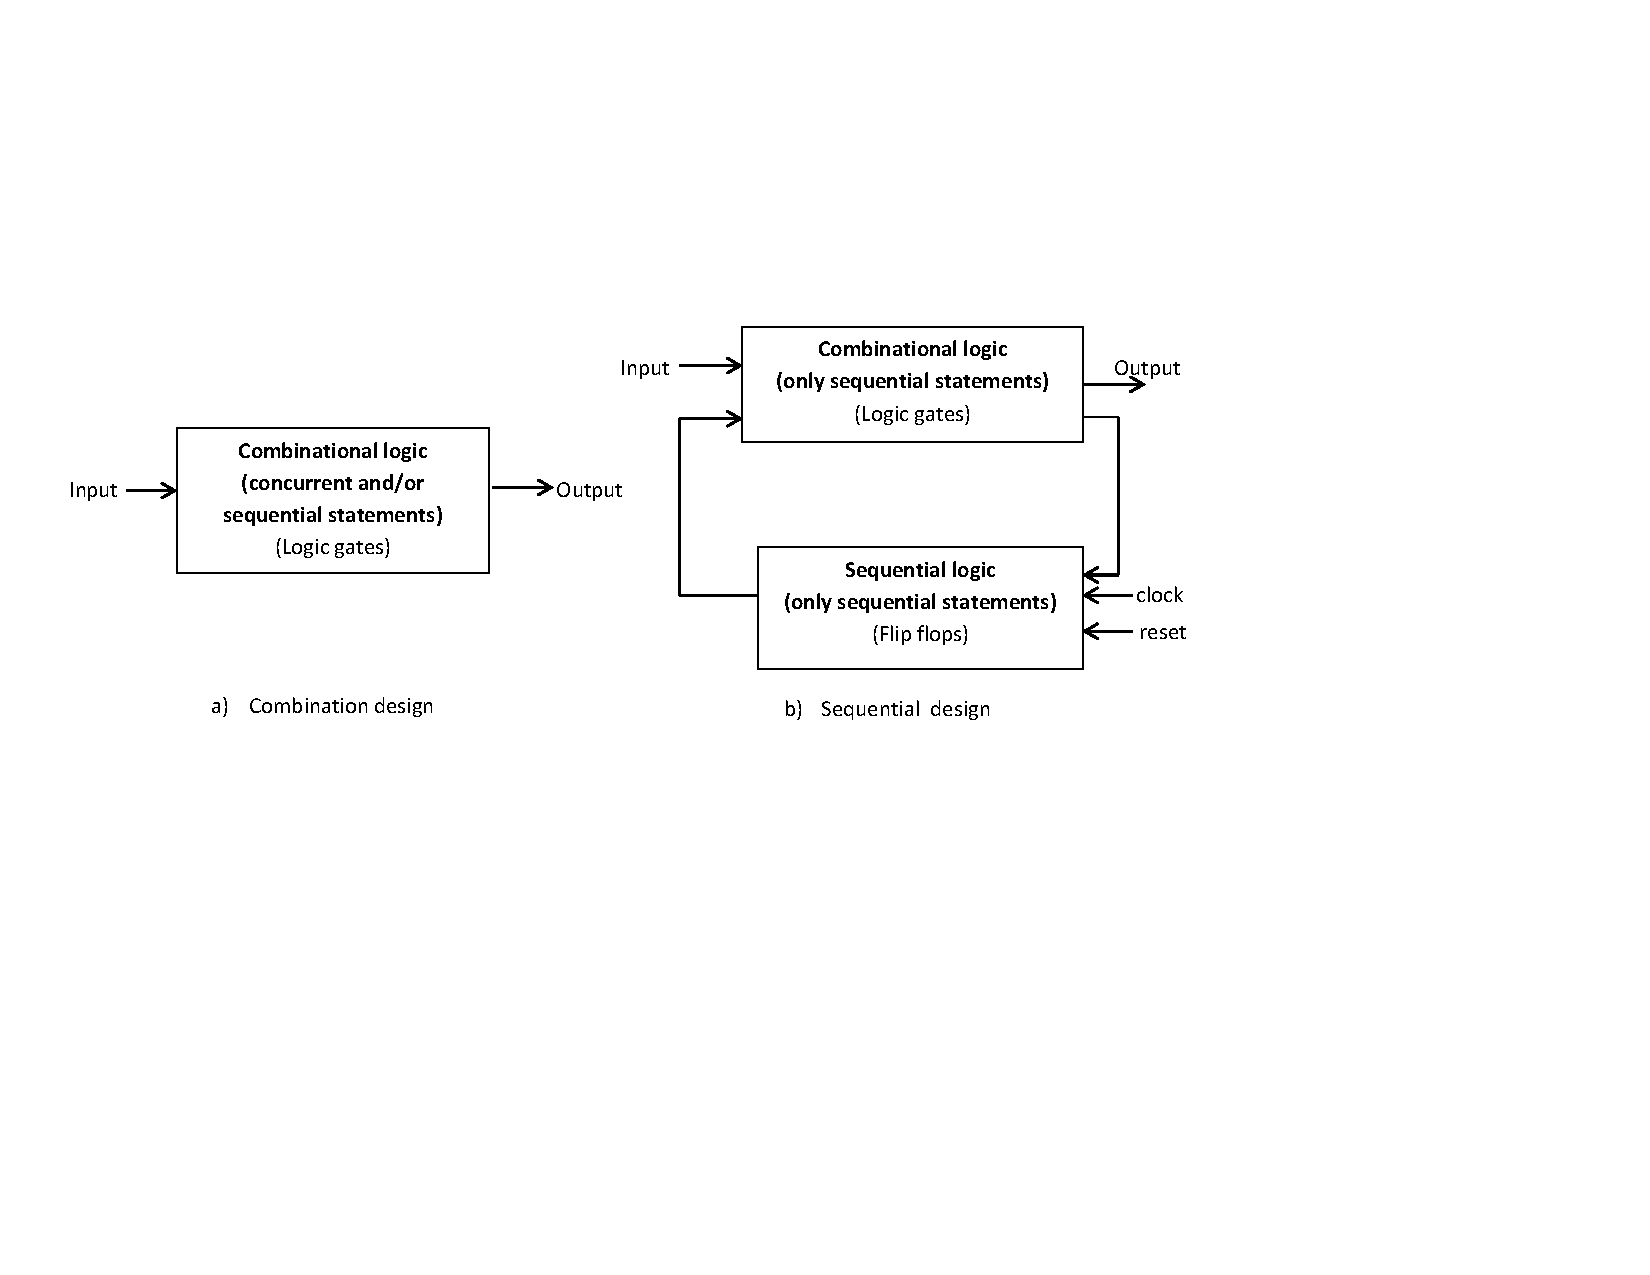
\includegraphics[scale=0.8]{combSeqBlock}
	\caption{Block diagram of `combinational' and `sequential' designs}
	\label{fig:combSeqBlock}
\end{figure}


\section{Concurrent statements and sequential statements}\label{sec:concurrentSeq}
\index{concurrent statements}\index{sequential statements}

In Listing \ref{verilog:comparator1Bit}, we saw that the concurrent statements execute in parallel, i.e. the order of the statement does not matter. Whereas Listing \ref{verilog:comparator2BitProcedure} shows the example of `sequential statements' where the statements execute one by one. Following are the relationship between `statements' and `design-type',

\begin{enumerate}
	\item Please note that `sequential statements' and `sequential designs' are two different things. Do not mix these together.
	\item Combinational designs can be implemented using both `sequential statements' and `concurrent statements'. 
	\item Sequential designs can be implemented using `sequential statements' only. 
	\item Sequential statements can be defined inside `always' block only. Further, these blocks executes concurrently e.g. if we have more than one always block then these block will execute in parallel, but statements inside each block will execute sequentially. 
	\item Sequential designs are implemented using various constructs e.g. `if', `case' and `for' etc., which are discussed in this chapter.
	\item Conditional operator (?:) can be used for combinational designs. 
\end{enumerate}

\begin{noNumBox}
	Remember : (see the words `design', `logic' and `statement' carefully) 
	\begin{enumerate}
		\item Only `logic gates (i.e. and, not and xor etc.)' are required to implement the combinational designs.
		\item Both `logic gates' and `flip flops' are required for implementing the sequential designs. 
		\item Lastly, the `sequential design' contains both `combinational logics' and `sequential logics', but the combinational logic can be implement using `sequential statements' only as shown in Fig. \ref{fig:combSeqBlock}; whereas the `combination logic' in the combinational designs can be implemented using both `concurrent' and `sequential' statements.
	\end{enumerate}
\end{noNumBox}

\section{`always' block}\index{always}
All the statements inside the always block execute sequentially. Further, if the module contains more than one always block, then all the always blocks execute in parallel, i.e. always blocks are the concurrent blocks. 

\begin{noNumBox}
	Note that, we can write the complete design using sequential programming (similar to C, C++ and Python codes). But that may result in very complex hardware design, or to a design which can not be synthesized at all. The best way of designing is to make small units using `continuous assignment statements' and `procedural assignment statements', and then use the structural modeling style to create the large system. 
\end{noNumBox}

\section{Blocking and Nonblocking assignment}
\index{blocking assignment}\index{nonblocking assignment}

There are two kinds of assignments which can be used inside the always block i.e. blocking and nonblocking assignments. The `=' sign is used in blocking assignment; whereas the `$<=$' is used for nonblocking assignment as shown in Listing \ref{verilog:blockAssignment} and \ref{verilog:nonblockAssignment}. Both the listings are exactly same expect the assignment signs at lines 13-14. Due to different in assignment signs, the design generated by these listings are different as shown in Fig. \ref{fig:blockingNonblockingAssg}, which are explained below.

\begin{explanation}[Listing \ref{verilog:blockAssignment}]
	In line 10, value of input port `x' is assigned to output `z'. Since, the value of `z' is equal to `x', therefore line 11 will be equivalent to `z = x + y'; due to this reason, the design is generated as `and' gate with inputs `x' and `y' as shown in Fig. \ref{fig:blockAssignment}.
\end{explanation}

\lstinputlisting[
language = Verilog,
caption    = {Blocking assignment, Fig. \ref{fig:blockAssignment}},
label      = {verilog:blockAssignment}
]{blockAssignment.v}


\begin{figure}[t!]
	\centering
	\begin{subfigure}[t]{0.5\textwidth}
		\centering
		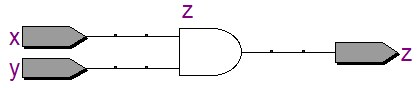
\includegraphics[scale=0.5]{blockAssignment}
		\caption{Blocking assignment, Listing \ref{verilog:blockAssignment}}
		\label{fig:blockAssignment}
	\end{subfigure}%
	\begin{subfigure}[t]{0.5\textwidth}
		\centering
		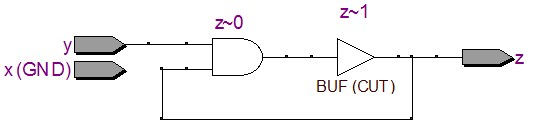
\includegraphics[scale=0.5]{nonblockAssignment}
		\caption{Nonblocking assignment, Listing \ref{verilog:nonblockAssignment}}
		\label{fig:nonblockAssignment}
	\end{subfigure}	
	\caption{Blocking and Nonblocking assignment}
	\label{fig:blockingNonblockingAssg}%
\end{figure}

\begin{explanation}[Listing \ref{verilog:nonblockAssignment}]
	\textbf{	In nonblocking assignment, updated values inside the block are not used for assignment.} In line 10, value of input port `x' is assigned to the `z'. Since updated value inside the block are not used in nonblocking assignment, therefore in line 11, `z = z $\&$ y;', the old value of `z' will be used for assignments (instead of z=x); hence a feedback path is used in Fig. \ref{fig:nonblockAssignment}. Also, `x' has no effect on the design as it is updating `z' inside the block, which will not be used by nonblocking assignment; hence `x' is not connected (i.e. connected to ground) in the design as shown in Fig. \ref{fig:nonblockAssignment}.
\end{explanation}

\lstinputlisting[
language = Verilog,
caption    = {Nonblocking assignment, Fig. \ref{fig:blockingNonblockingAssg}},
label      = {verilog:nonblockAssignment}
]{nonblockAssignment.v}

\section{Guidelines for using `always' block} \label{sec:guideAlwaysblock}\index{always!guidelines for usage}
The general purpose `always' block of Verilog can be misused very easily. And the misuse of this block will result in different `simulation' and `synthesis' results. In this section, the general guidelines are provided for using the `always' block in different conditions. Further, it is better to use the specilialized `always' blocks of SystemVerilog to avoid the ambiguities in synthesis and simulation results, which are discussed in Section \ref{sec:specialAlwaysBlk}. 

\begin{noNumBox}
	Note that, the `always' block is used for `synthesis (i.e. with sensitive list)' as well as `simulation (i.e. with and without sensitive list)', which have different set of semantic rules. If we do not follow the below guidelines in the designs, then simulation and synthesis tools will infer different set of rules, which will result in differences in synthesis and simulation results. Further, SystemVerilog has specialized `always blocks' for different types of designs (see Section \ref{sec:specialAlwaysBlk}), which can catch the errors when the designs are not created according to below rules. 
\end{noNumBox}
\subsection{`always' block for `combinational designs'}
Follow the below rules for combinational designs, 
\begin{enumerate}
	\item Do \textbf{not} use the `posedge' and `negedge' in sensitive list. 
	\item Sensitive list should contain all the signals which are read inside the block. 
	\item No variable should be updated outside the `always' block. 
	\item Use \textbf{blocking assignment (i.e. = )} for assigning values. 
	\item All the variables should be updated for all the possible input conditions i.e. if-else and case statements should include all the possible conditions; and all the variables must be updated inside all the conditions. 
\end{enumerate}

\subsection{`always' block for `latched designs'}
Follow the below rules for latched designs, 
\begin{enumerate}
	\item Do \textbf{not} use the `posedge' and `negedge' in sensitive list. 
	\item Sensitive list should contain all the signals which are read inside the block. 
	\item No variable should be updated outside the `always' block. 
	\item Use \textbf{blocking assignment (i.e. = )} for assigning values. 
	\item At least one the variables should \textbf{not} be updated for some of the possible input conditions.
\end{enumerate}

\subsection{`always' block for `sequential designs'}
Follow the below rules for sequential designs, 
\begin{enumerate}
	\item \textbf{Use} either `\textit{posedge}' or `\textit{negedge}' (not both) in sensitive list for all the elements. 
	\item No variable should be updated outside the `always' block. 
	\item Use \textbf{non-blocking assignment (i.e. $<=$ )} for assigning values. 
\end{enumerate}


\section{If-else statement} \label{sec:ifElse}\index{if-else}
In this section, a 4$\times$1 multiplexed is designed using If-else statement. We already see the working of `if' statement in the Chapter \ref{ch:OverView}. In lines 11-24 of Listing \ref{verilog:ifEx}, `else if' and `else' are added to `if' statement. Note that, If-else block can contain multiple `else if' statements between one `if' and one `else' statement. Further, `begin - end' is added in line 12-15 of Listing \ref{verilog:ifEx}, which is used to define multiple statements inside `if', `else if' or `else' block.  Fig. \ref{fig:ifExWave} shows the waveform generated by Modelsim for Listing \ref{verilog:ifEx}. 
Note that, we are generating the exact designs as the VHDL tutorials, therefore line 22-23 are used. Also, we can remove the line 22-23, and change line 20 with `else', which will also work correctly. 

\begin{figure}[!h]
	\centering
	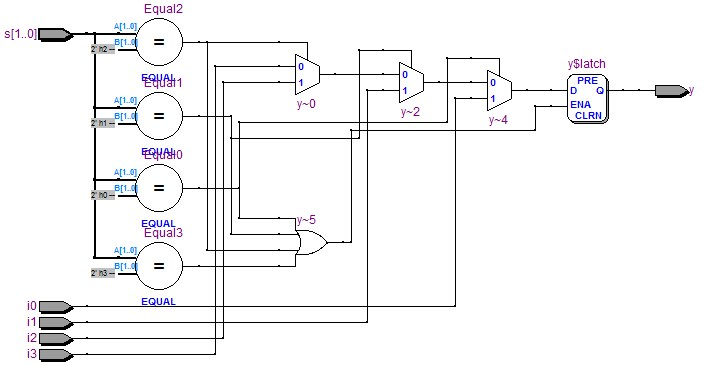
\includegraphics[width=0.8\textwidth]{ifEx}
	\caption{Multiplexer using if statement, Listing \ref{verilog:ifEx}}
	\label{fig:ifEx}
\end{figure} 

\lstinputlisting[
language = Verilog,
caption    = {Multiplexer using if statement},
label      = {verilog:ifEx}
]{ifEx.v}

\begin{figure}
	\centering
	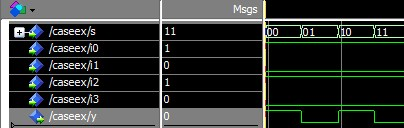
\includegraphics[scale=1]{ifExWave}
	\caption{Waveforms of Listing \ref{verilog:ifEx} and \ref{verilog:caseEx}}
	\label{fig:ifExWave}
\end{figure}
%
%
%
%
\section{Case statement}\index{case}
Case statement is shown in lines 11-16 of Listing \ref{verilog:caseEx}. `s' is used in case statement at line 11; whose value is checked using `when' keyword at lines 12 and 13 etc. The value of the output y depends on the value of `s' e.g. if `s' is `1', then line 12 will be true, hence value of `i1' will be assigned to `y'. Note that, we can use `integer' notation (line 12) as well as `binary' notation (line 13)  in `case' and `if' statements. Design generated by Listing \ref{verilog:caseEx} is shown in Fig. \ref{fig:caseEx}.

\lstinputlisting[
language = Verilog,
caption    = {Multiplexer using case statement},
label      = {verilog:caseEx}
]{caseEx.v}
\begin{figure}[!h]
	\centering
	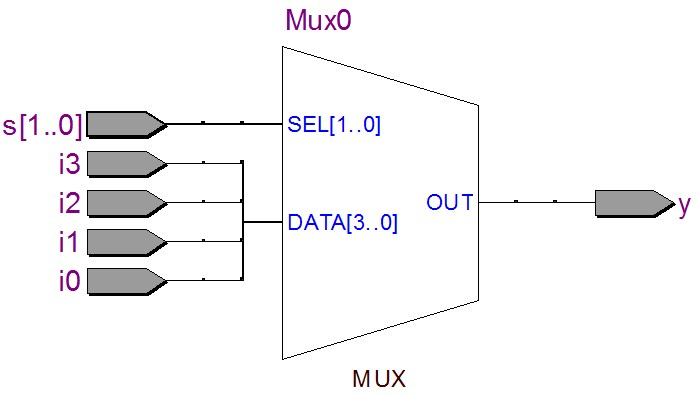
\includegraphics[scale=0.4]{caseEx}
	\caption{Multiplexer using case statement, Listing \ref{verilog:caseEx}}
	\label{fig:caseEx}
\end{figure}

We need not to define all the possible cases in the `case-statement', the ``default'' keyword can be used to provide the output for undefined-cases as shown in Listing \ref{verilog:caseEx2}. Here, only two cases are defined i.e. 7 and 3; for the rest of the cases, the default value (i.e. i2) will be sent to the output. 

\lstinputlisting[
language = Verilog,
caption    = {Case-statement with default values},
label      = {verilog:caseEx2}
]{caseEx2.v}

\section{Problem with Loops}

Verilog provides two loop statements i.e. `for' loop and `while' loop'. These loops are very different from software loops. Suppose `for i = 1 to N' is a loop', then, in software `i' will be assigned one value at time i.e. first i=1, then next cycle i=2 and so on. Whereas in Verilog, N logics will be implement for this loop, which will execute in parallel. Also, in software, `N' cycles are required to complete the loop, whereas in Verilog the loop will execute in one cycle. 
\begin{noNumBox}
	As loops implement the design-units multiple times, therefore design may become large and sometimes can not be synthesized as well. If we do not want to execute everything in one cycle (which is almost always the case), then loops can be replaced by `case' statements and `conditional' statements as shown in section \ref{sec:ifLoop}. Further, due to these reasons, we do not use loops in the design, and hence these are not discussed in the tutorial.
\end{noNumBox}   
%
\section{Loop using `if' statement}\label{sec:ifLoop}
In Listing \ref{verilog:ifLoop}, a loop is created using `if' statement, which counts the number upto input `x'. 

\begin{explanation}[Listing \ref{verilog:ifLoop}]
	In the listing, two `always' blocks are used i.e. at lines 20 and 33. The process at line 20 checks whether the signal `count' value is `less or equal' to input x (line 22), and sets the currentState to `continueState'; otherwise if count is greater than the input x, then currentState is set to `stopState'.
	
	Then next `always' statement (line 33), increase the `count' by 1, if currentState is `continueState'; otherwise count is set to 0 for stopState. Finally count is displayed at the output through line 41. In this way, we can implement the loops using the `always' statements. 
	
	Fig. \ref{fig:ifLoop} shows the loop generated by the listing with parameter N=1. Further,  Fig. \ref{fig:ifLoopWave} shows the count-waveforms generated by the listing with parameter N = 3.
\end{explanation}
%
\lstinputlisting[
language = Verilog,
caption    = {Loop using `if' statement},
label      = {verilog:ifLoop}
]{ifLoop.v}
\begin{figure}[!h]
	\centering
	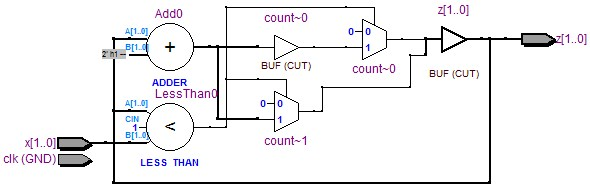
\includegraphics[scale=0.85]{ifLoop}
	\caption{Loop using `if' statement, Listing \ref{verilog:ifLoop} with N = 1}
	\label{fig:ifLoop}
\end{figure}

\begin{figure}[!h]
	\centering
	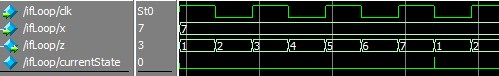
\includegraphics[width=\textwidth]{ifLoopWave}
	\caption{Loop using `if' statement, Listing \ref{verilog:ifLoop} with N = 3}
	\label{fig:ifLoopWave}
\end{figure}
%
\begin{noNumBox}
	Sensitivity list of the always block should be implemented carefully. For example, if we add `count' in the sensitivity list at line 33 of Listing  \ref{verilog:ifLoop}, then the always block will execute infinite times. This will occur because the always block execute whenever there is any event in the signals in the sensitivity list; therefore any change in `count' will execute the block, and then this block will change the `count' value through line 36. Since `count' value is changed, therefore always block will execute again, and the loop will never exit.  
	\\ \\
	Another problem is that,  above error can not be detected during simulation phase, i.e. simulation will show the correct results. Such errors are very difficult to find in Verilog. Further, such errors can be identified in VHDL code, as shown in VHDL tutorials. To avoid such errors in Verilog, please follow the guidelines for using the `always' block as described in Section \ref{sec:guideAlwaysblock}. 
\end{noNumBox}
%
\section{Conclusion}
In this chapter, various statements for procedural assignments are discussed. Problem with loops are discussed and finally loop is implemented using `if' statement. Lastly, it is shown that, Verilog designs can have differences in simulation results and implementation results. 

